\documentclass[
  coverheight=9.861in,
  spinewidth=1.375in,
  bleedwidth=0.306in,
  11pt,
  trimmed
]{bookcover}

\usepackage{lettrine}
\usepackage{fancybox}
\usepackage{wrapfig}
\usepackage[T1]{fontenc}
\usepackage{Alegreya} %% Option 'black' gives heavier bold face 

\newcommand{\olpath}{../}
\newcommand{\whitebg}[1]{%
\tikz\node[circle,draw,minimum size=.9cm,
fill=white,
path picture={
    \node at (path picture bounding box){
        \includegraphics[width=.9cm]{\olpath#1}
    };
}]{};
}

% \newcommand{\tikzcircle}[2][red,fill=red]{\tikz[baseline=-0.5ex]\draw[#1,radius=#2] (0,0) circle ;}%


\definecolor{BackgroundColor}{HTML}{f3f6ed}
\definecolor{SpineBackColor}{HTML}{262626}
\definecolor{SpineFontColor}{RGB}{248,154,14}

\begin{document}

\begin{bookcover}
  \bookcovercomponent{color}{bg whole}{color=BackgroundColor}
  \bookcovercomponent{color}{spine}{color=SpineBackColor}
  \bookcovercomponent{normal}{front}{
  \vspace{2.5cm}
  \begin{center}
    \fontsize{40pt}{7em}\selectfont\bfseries
        CATEGORY THEORY \\FOR PROGRAMMERS
    \vfil
    \hspace*{-1cm}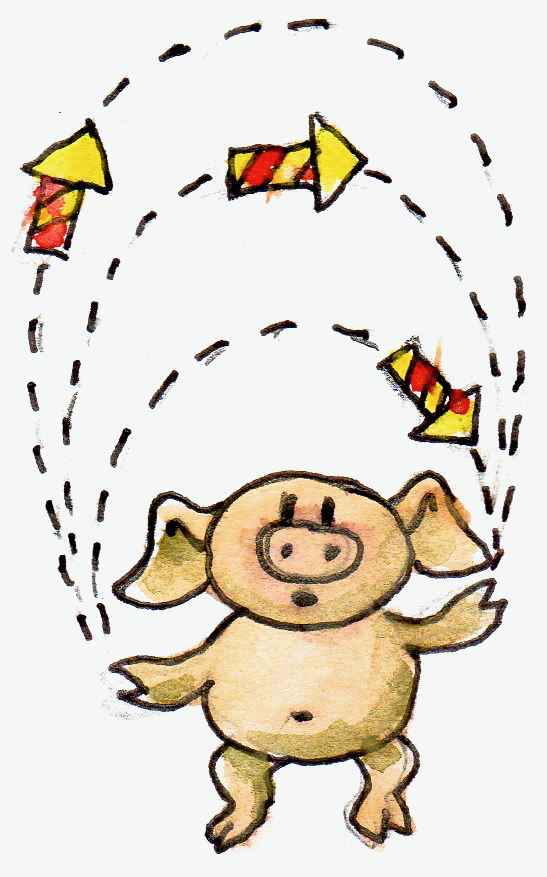
\includegraphics[width=8cm]{./piggie.png}%
    \vfil
    \normalfont\Huge
    \textbf{Bartosz Milewski}
    \vfil
    \vspace*{1cm}
  \end{center}}
  \bookcovercomponent{center}{spine}{
    \rotatebox[origin=c]{-90}{\color{SpineFontColor}\bfseries\Huge Category Theory for Programmers \hspace{2em} Bartosz Milewski}}
  \bookcovercomponent{normal}{back}{
    \centering
    \vspace{1mm}
    \begin{figure}[H]
      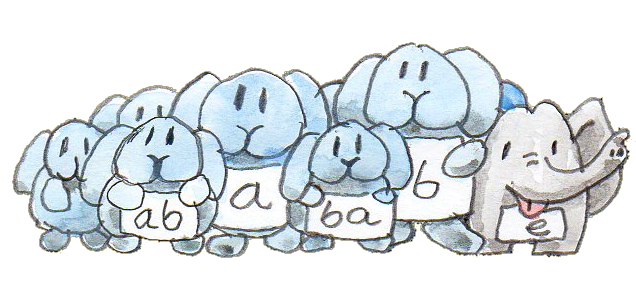
\includegraphics[width=120mm]{bunnies.png}
    \end{figure}
    \parbox{130mm}{\color{black}
      \Large
      \lettrine[lhang=0.17]{C}{ategory Theory}
      is one of the most abstract branches of mathematics. It is usually taught to
      graduate students after they have mastered several other branches of mathematics,
      like algebra, topology, and group theory. It might therefore come as a shock that
      the basic concepts of category theory can be explained in relatively simple terms
      to anybody with some experience in programming. \\
      
      That's because, just like programming,
      category theory is about structure. Mathematicians discover structure in mathematical
      theories, programmers discover structure in computer programs. Well structured programs
      are easier to understand and maintain, and are less likely to contain bugs. Category
      theory provides the language to talk about structure, and learning it will make you
      a better programmer.
    \rule{130mm}{0.4pt}
    \begin{tabular}[h]{p{3.6cm} p{10cm}}
      \vspace{0pt}
      \begin{figure}[H]
        \centering
        \shadowsize=2pt
        \fboxrule=0pt
        \fboxsep=0pt
        \color{gray}
        \shadowbox{\fboxsep=1pt
\includegraphics[height=40.5mm]{bartosz.jpg}}
      \end{figure}
      &
      \vspace{0pt}
      \begin{minipage}[b]{8.5cm}
        \fontsize{11pt}{1.4em}\selectfont\textit{Category Theory for Programmers}
          by Bartosz Milewski is licensed under a Creative Commons Attribution 4.0
          International License.\\
      \break
      \begin{minipage}[b]{4cm}
        \whitebg{/fig/icons/by}
        \whitebg{/fig/icons/cc}
        \whitebg{/fig/icons/sa}
      \end{minipage}
  
      \break
      Edited by Igal Tabachnik
      \end{minipage}
    \end{tabular}}}
  
\end{bookcover}
\end{document}